\chapter{Effects of Network Topology}

\section{Node Distance from the Anchors}

Of great assistance to network designers is to know which regions of the network to expect poor localization performance.  With this information, and if the anchor placement is constrained, they could either avoid placing nodes in the expected poor area, or take into account the higher expected localization errors in the analysis of the data.

Figure~\ref{fig:AS6goodcontour} shows a different view of in-network errors. Instead of showing a line representing the localization errors as in other figures present in this study, the error at each node is used to interpolate and a grid of location errors is throughout the area of the network.  A contour plot based on that interpolated grid is then shown in the figure.  The goal in viewing the network map in this way is to discover a pattern in terms of the relationship of a an area of the network to the location of the anchor nodes themselves.  Unfortunately, no geographic correlation between location error and anchor node placement can be ascertained.  It may be possible, with future study, to remove the effect of other factors to reveal a pattern based on anchor placement.

\begin{figure}
  \centering
	\subfloat[Network A]{
		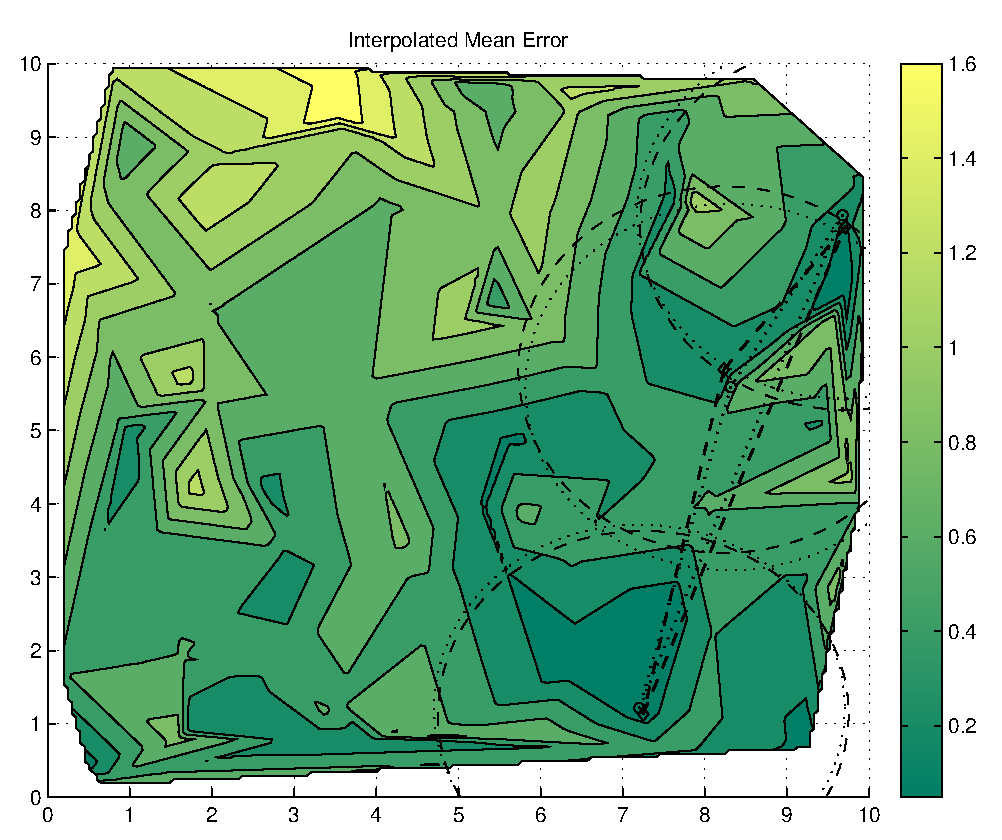
\includegraphics[width=\figurewidth\textwidth]{outliers/AS6/AS6NetworkContour7}}
	\\
	\subfloat[Network B]{
		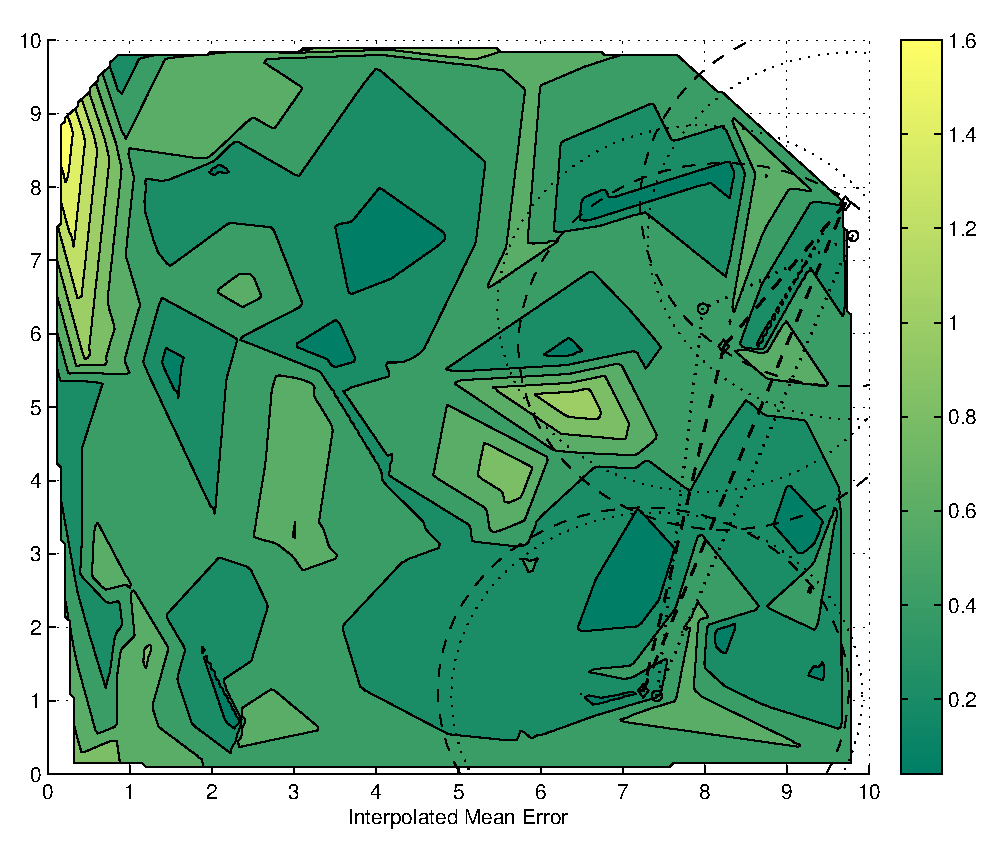
\includegraphics[width=\figurewidth\textwidth]{outliers/AS6/AS6NetworkContour10}}
	\caption{Localization error as a contour plot}
	\label{fig:AS6goodcontour}
\end{figure}


\section{Applicability to Varying Network Topologies}

So far, we have examined anchor node placement for a continuous square network, with randomly placed nodes.  However, in the real world, networks are not alway so simple.  There are often regions in the network where it is not possible to put nodes, due to physical barriers like lake, buildings or access to property.  In this section, we look at how the results thus far apply to C-shaped and long, narrow pipeline network topologies.

\subsection{C-Shape Network Topology}

A C-shape network consists of a relatively square region with an empty area on one side, as shown in Figure~\ref{fig:cnetwork}.  In terms of anchor placement requirements, we do not expect any difference between the recommendations presented for square networks.

\begin{figure}
  \centering
	\includegraphics[width=\textwidth]{cshape/network}
	\caption{Example of C-shape network topology}
	\label{fig:cnetwork}
\end{figure}

To show that there is no difference, 10 random networks with 5000 anchor sets each was simulated in the same manner as the square networks.  Figure~\ref{fig:cindicator} shows the location error relative to the sum of the distances between the anchors, as in Section~\ref{sec:bestanchornode}. 
As expected, the mean location error flattens out as the sum of distances between anchor nodes reaches about 10 times the radio range.  There is a slight increase in the mean location error as compared with the square network, but this has to do with the performance of the CCA algorithm itself with the presence of the empty region of nodes in the network.  The increase in mean location error at the end of the plot, and specifically the increase in the confidence interval, is caused by the small sample size in the random selection of anchor set with very high distance between nodes. 

\begin{figure}
  \centering
	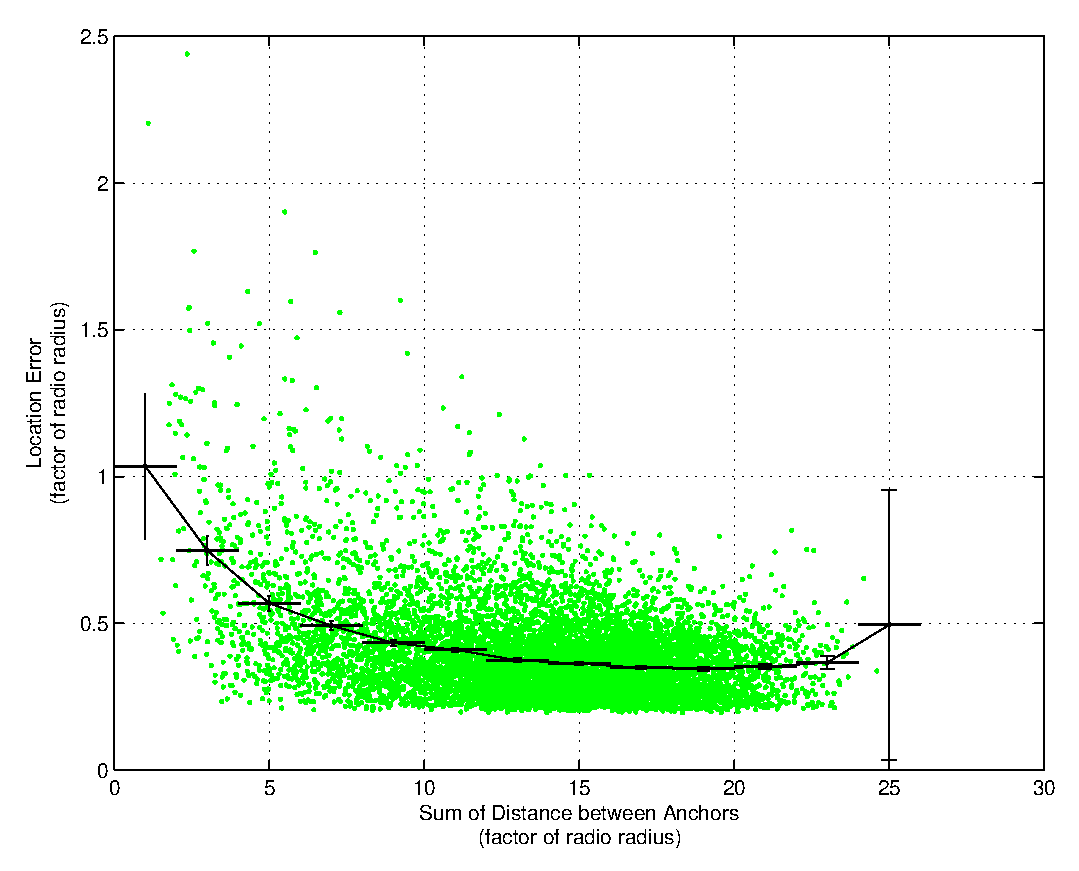
\includegraphics[width=\textwidth]{cshape\SumOfDistanceIndicator_cshape}
	\caption[Sum of distance between anchors vs location error in a C-Shape topology]{Sum of distance between anchors vs location error for 10 random C-shape 20-by-20 unit networks with 400 nodes, 5000 anchor sets each, and a radio range of 2.5 units, excluding outliers}
	\label{fig:cindicator}
\end{figure}

\subsection{Pipeline Network Topology}

In some applications, that network region has very little depth to it, such as a long pipeline or along a highway or railroad line.  The extreme case is where there is a single node placed along a straight axis.  As we have shown, this is the worst possible scenario, as it is the most likely was to cause the outlier condition for localization.  In that case, it is worthwhile to explore the possibility of other localization techniques, such as GPS at each node, or recording the location as the nodes are placed.  

However, for randomly nodes, when there is a bit of depth to the network, as shown in Figure~\ref{fig:pipeline} (not equal x and y scales), there is still the possibility of good localization results.  As before, a simulation was run.  However, for pipeline networks with randomly placed nodes, it is much more difficult to meet the network connectivity requirements.  Therefore, the simulations are run for just six networks with 400 nodes in a 200x2 unit area.  Note that the height of the network, 2 units, is less than the radio range, 2.5 unites.  Also recall that the recommendation to avoid outliers is that the minimum height of the triangle must be a least one times that radio range, which even the height of the network does not meet this criteria. 

Even worse than expected, all of the 30,000 anchor sets across the six networks are outlier cases.  Figure~\ref{fig:pipelineindicator} shows that that the mean location error is about 18 times the radio range which is well beyond any reasonable value.

\begin{figure}
  \centering
	\includegraphics[width=\textwidth]{pipeline/network}
	\caption{Example of pipeline network topology}
	\label{fig:pipeline}
\end{figure}

\begin{figure}
  \centering
	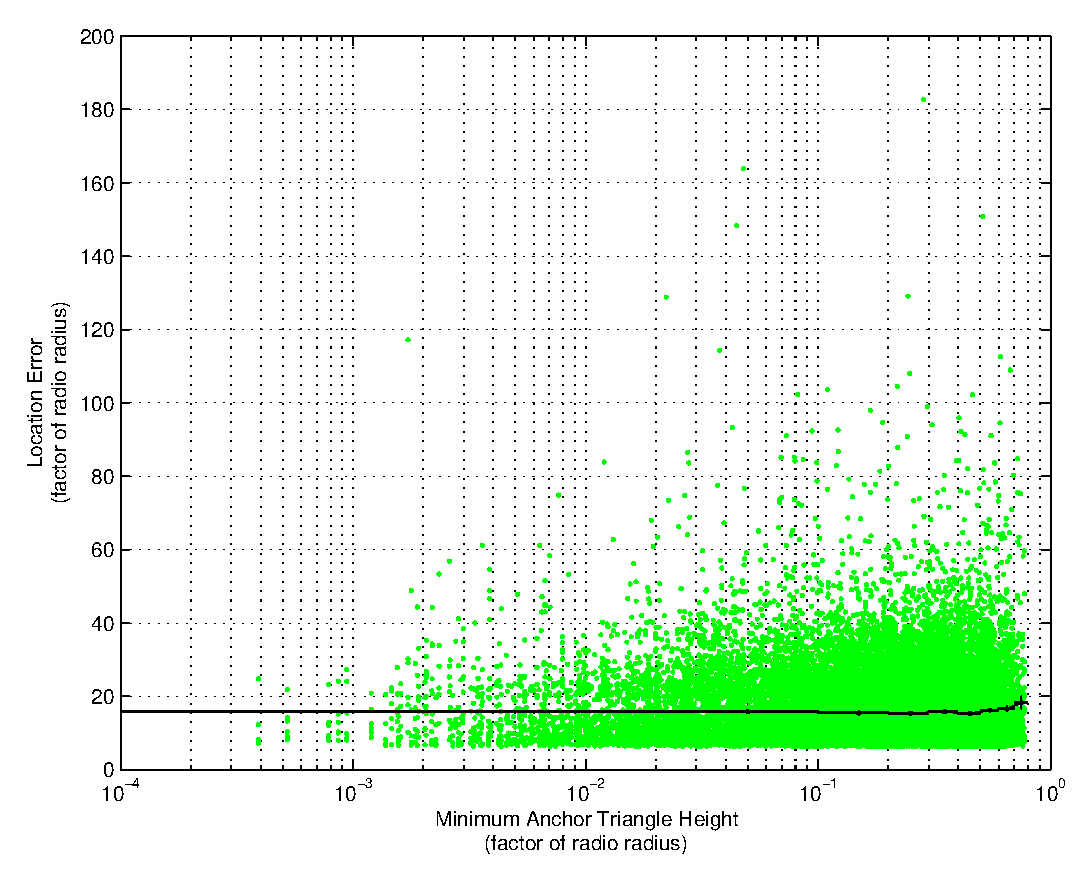
\includegraphics[width=\textwidth]{cshape\HeightIndicator_pipeline}
	\caption[Minimum height of the triangle formed by the anchor nodes vs location error in a pipeline topology]{Minimum height of the triangle formed by the anchor nodes vs location error for 6 random pipeline 200-by-2 unit networks with 400 nodes, 5000 anchor sets each, and a radio range of 2.5 units}
	\label{fig:pipelineindicator}
\end{figure}
